\subsection{Plutonium Redistribution}

As a consequence of restructuring, it became necessary to investigate the phenomenon of Plutonium redistribution. During restructuring, distinct zones form within the fuel element:

\begin{itemize}
    \item \textbf{Central void}: Pores migrate, leading to mass displacement outward.
    \item \textbf{Columnar grains}: Caused by pore migration and density changes.
    \item \textbf{Equiaxed grains}: Formed by grain growth at high temperatures.
    \item \textbf{As-fabricated zone}: A region where the temperature is too low to cause significant changes.
\end{itemize}

These zones exhibit differences in density and porosity, with the fuel reaching up to 98-99\% of its theoretical density (TD). This density variation leads to a redistribution of Plutonium concentration across the zones, which initially had a uniform concentration of 29\%. 

Plutonium becomes enriched in the central (columnar) zone, followed by a decrease (reaching a minimum) in the equiaxed zone. In the as-fabricated zone, the concentration stabilizes back to the initial value. This redistribution is driven by Plutonium’s high activation energy, which enables migration within the fuel.

To evaluate how Plutonium redistribution varies due to thermal expansion and restructuring, we employed the following formula (from the provided handouts, Hot Effects Analysis, V):

\begin{equation}
    \frac{q'''(r)}{q_0} = \frac{c(r)}{c_0} = 1 + D \left\{ 
    \exp \left[ -2 \alpha \left( \frac{r - r^*}{R_\text{fo}} \right) \right] 
    - 2 \cdot \exp \left[ -\alpha \left( \frac{r - r^*}{R_\text{fo}} \right) \right]
    \right\}
\end{equation}

where:
\begin{itemize}
    \item $D = 0.01$: Redistribution factor (from handouts),
    \item $\alpha = 10$: Exponential parameter (from handouts),
    \item $r^* = 0.207 \cdot R_\text{fo}$: Empirical constant ensuring conservation of Plutonium,
    \item $c(r)$: Radial Plutonium concentration [g/cm\(^3\)],
    \item $c_0$: Initial Plutonium concentration.
\end{itemize}

This equation models the radial variation of Plutonium concentration, accounting for the interplay of thermal and structural effects. Graphically, the results highlight the key phenomena associated with Plutonium redistribution.

Figure~\ref{fig:Redistribution_Structure} illustrates the restructuring of the fuel element and the formation of distinct zones during irradiation. Figure~\ref{fig:Pu_Profile} shows the radial Plutonium concentration profile, normalized relative to the initial concentration.

\begin{figure}[H]
\centering
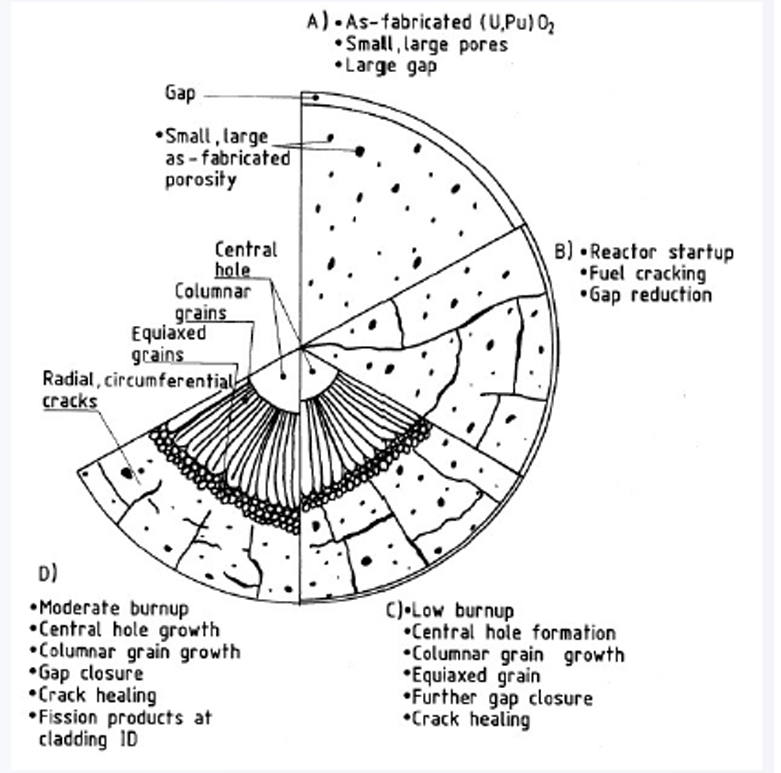
\includegraphics[width=0.6\textwidth]{Pu_redistributio_explaination.png}
\caption{Restructuring of fuel elements and formation of zones during irradiation.}
\label{fig:Redistribution_Structure}
\end{figure}

\begin{figure}[H]
\centering
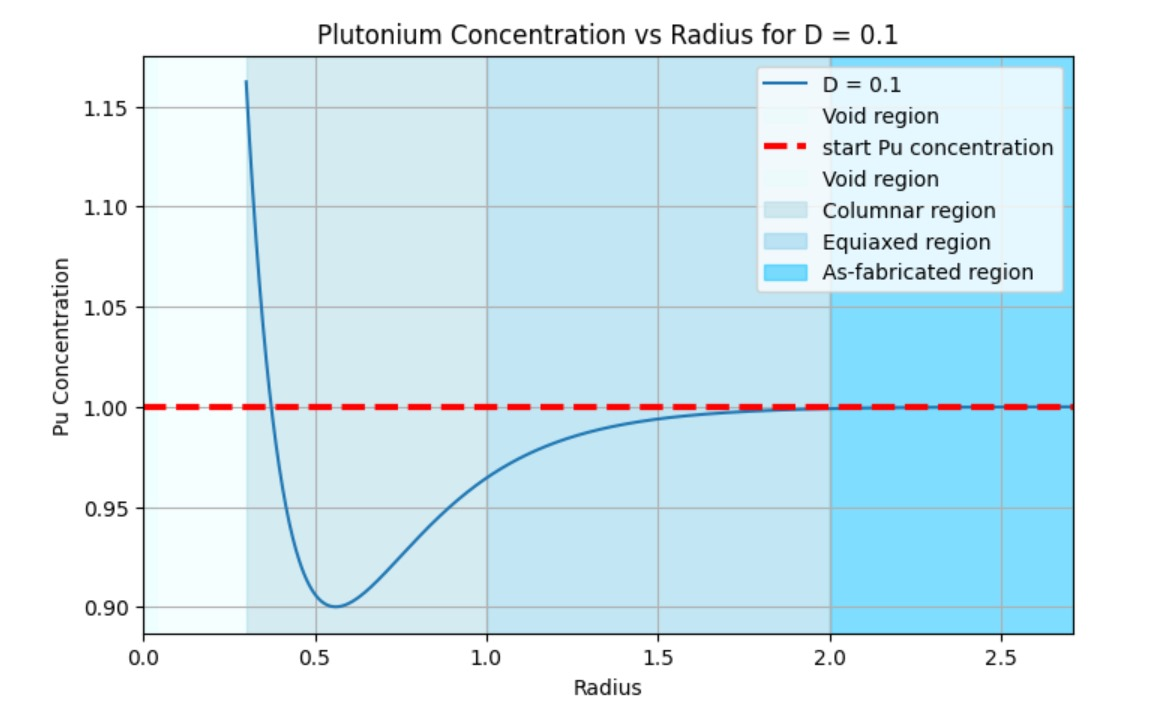
\includegraphics[width=0.8\textwidth]{Pu_redistribution_profile.jpg}
\caption{Radial distribution of Plutonium concentration (relative to the starting concentration) within the fuel structure.}
\label{fig:Pu_Profile}
\end{figure}
